\chapter{Hardware}

The hardware comprising the embedded system in \ref{fig:rwm} is based on a master-slave configuration.


\section{Theory of operation}
\label{sec:Too}


\subsubsection{Master-Slave microcontroller configuration}

We use a pair of 32-bit microcontroller to capture and transmit data collected from the water meter.
The reason for this configuration stems from the fact that we were unable to completely switch off the GSM module on the
Arduino MKR GSM 1400 development kit (DK) which resulted in more energy consumption than we can meet with the off-grid solution
we have described in the last
section.
Thus, the master controls the infrared sensor, digitizes the sensor signal and accumulates a counter which it transmits to the
slave. The slave
transmits the data during selected time slots. The master controls power to the slave and the latter
is completely switched off outside of transmission intervals. We will discuss further details of the pro and cons of this configuration later in
this article.



\begin{figure}[h]
    \centering
    \begin{subfigure}[b]{0.45\textwidth}
        \centering
        \includegraphics[width=.8\linewidth]{mkrzero}
        \subcaption{Master: Arduino MKR Zero DK}
        \label{fig:x}
    \end{subfigure}
    \hfill
    \begin{subfigure}[b]{0.45\textwidth}
        \centering
        \includegraphics[width=.8\linewidth]{mkrgsm}
        \subcaption{Slave: Arduino MKR GMS 1400 DK}
        \label{fig:x}
    \end{subfigure}
    \caption{Master slave embedded system configuration}
    \label{fig:x}
\end{figure}
\subsubsection{Master-Slave handshake operation}

The master increments a counter on each high-low transition of the phototransistor's collector voltage.
This value is accumulated during 24 hours and then uploaded to a server that is accessible via the Internet.
Since the upload is done by the slave, the counter value must be transferred to the slave (via I2C).
Once this value has been successfully transferred, the slave sends a success code to the master and the counter
is updated with the number of increments that  occurred between the request to the slave and the reply from the slave.
\par

In case the data could not be transferred within in a given budget of attempts, the slave sends a failure code.
In either case the slave is shutdown by the master after the reply has been received.
In case of failure, the master will not reset the counter and start
another transmission attempt later.
The slave might also get stuck while attempting to transmit data. In this case, the slave firmware makes no progress and no
reply is sent to the master. To avoid a deadlock, the master will simply switch of the slave after a given delay and consider
the transmission attempt as failed.
\par
The transmission is done via the I2C bus.
Once the slave is powered on, it will connect its I2C interface with the one of the master controller via analog switches.
This allows data to be exchanged in both directions.
The analog switches provide I2C bus isolation. Since the slave controller can be powered of while the master controller is
powered on, the former would  be back-powered via the I2C IO pins through the internal
ESD diode. This situation can cause malfunctions and violates the Absolute Maximum Ratings of the SAMD21 microcontroller
hosted on the Arduino DKs.
This situation must therefore be avoided.


\section{Module structure}


In the following section, we present the embedded system hardware as a set of modules.
Modules can be composed of hardware components like resistors or integrated circuits (IC).
A module can also contain other modules in a nested, tree-like structure.

Modules are interconnected with nets. Nets are labeled, for example \textit{5V} or \textit{B}.
A net is labeled  in the module where it first occurs in a top-down manner. It can then been referred to
in a child module by prepending a dot to the label. For example, given that net \textit{\emph{B}} has been introduced
in the top-level module, it will be referred to as \textit{\emph{.B}} in any child module.
This notation is inspired from object-oriented programming.
A net has also an Id and a Rank. The former is a sequential number starting at 1 that is local to each module.
Rank is a hint on how important the net is when it comes to PCB layout. For example, nets carrying high-speed signals
or supply power are usually higher ranked than a net that controls a user LED.


\clearpage
\section{Remote Water Meter (RWM) system}

The RWM system is composed of four top-level modules:

\begin{enumerate}
    \item Master Module (MA): water flow measurement and SL power management.
    \item Slave Module (SL): data transmission via GSM.
    \item Power Module (PO): power source aggregation, signal conditioning and MA power management.
    \item Optical Sensor (OS): signal conditioning of water flow indicator (tally).
\end{enumerate}

\begin{figure}[h]
    \centering
    \includegraphics[width=1.0\textwidth]{EP}
\end{figure}


\begin{table}[H]
    \centering
    \begin{threeparttable}[b]
        \begin{tabularx}{\linewidth}{ >{\hsize=0.15\hsize}X > {\hsize=0.15\hsize}X > {\hsize=0.25\hsize}X >{\hsize=3.45\hsize}X}
            Id & Rank & Name                   & Net description                                                                            \\
            \midrule
            1  & 5    & S\textsubscript{1}     & solar panel 1, positive output voltage                                                     \\
            2  & 5    & S\textsubscript{2}     & solar panel 2, positive output voltage                                                     \\
            3  & 5    & S\textsubscript{1'}    & V\textsubscript{s1}  protected against overvoltage                                         \\
            4  & 5    & S\textsubscript{2'}    & V\textsubscript{s1}  protected against overvoltage                                         \\
            17 & 5    & S\textsubscript{'\lor} & S\textsubscript{1'} OR S\textsubscript{2'}, OR-ing of dual solar power sources             \\
            5  & 2    & 5V                     & USB compatible charger output                                                              \\
            6  & 1    & B                      & battery voltage                                                                            \\
            6  & 1    & B'                     & scaled down battery voltage for \SI{3.3}{\V} A/D conversion                                \\
            7  & 3    & V\textsubscript{\mu M} & supply voltage  for master microcontroller (\mu M) controlled by the Power Module (PO).    \\
            8  & 6    & S\textsubscript{1'c}   & scaled down V\textsubscript{s1'} for \SI{3.3}{\V} A/D conversion                           \\
            9  & 6    & S\textsubscript{2'c}   & scaled down V\textsubscript{s2'} for \SI{3.3}{\V} A/D conversion                           \\
            10 & 2    & \texttt{SDA}           & slave: I2C data                                                                            \\
            11 & 2    & \texttt{SCL}           & slave: I2C clock                                                                           \\
            12 & 2    & V\textsubscript{\mu S} & supply voltage for slave microcontroller                                                   \\
            13 & 2    & \texttt{CON}           & slave: are slave I2C bus and master I2C  connected ?                                       \\
            14 & 2    & \texttt{ACK}           & slave: is slave  ready to receive I2C data from master   ?                                 \\
            15 & 2    & V\textsubscript{OS}    & supply voltage for Optical Switch (OS) module controlled by \mu M.                         \\
            16 & 2    & Prx                    & optical sensor output voltage (position of water meter tally) for A/D conversion by \mu C. \\
        \end{tabularx}
    \end{threeparttable}
\end{table}

\clearpage



\clearpage
\section{Master Module (MA)}

The MA module is composed of six modules:

\begin{enumerate}
    \item Display (DP): present process info to the user.
    \item Watchdog Timer (WD): supervise program flow of \mu M.
    \item Slave Switch (SS) : control power supply to Slave Module (SL).
    \item \mu C Master (\mu M): run the water flow measurement firmware.
    \item Bus Isolation (BI$_1$, BI$_2$): prevent back-powering via GPIO and I2C when SL is switched off.
    \item Opto Switch Driver (OD): control power supply to the Optical Sensor Module (OS).
\end{enumerate}


\begin{figure}[h]
    \centering
    \includegraphics[width=1.0\textwidth]{MA/MA}
\end{figure}


\begin{table}[H]
    \centering
    \begin{threeparttable}[b]
        \begin{tabularx}{\linewidth}{ >{\hsize=0.15\hsize}X >
                    {\hsize=0.15\hsize}X > {\hsize=0.25\hsize}X >{\hsize=3.45\hsize}X}
            Id & Rank & Name             & Net description                                            \\
            \midrule
            1  & 1    & 3.3V             & voltage provided by \mu M                                  \\
            3  & 4    & \texttt{ESS}     & enable SS                                                  \\
            4  & 4    & \texttt{CON'}    & slave: are slave I2C bus and master I2C  connected ?       \\
            5  & 4    & \texttt{ACK'}    & slave: is slave  ready to receive I2C data from master   ? \\
            6  & 4    & \texttt{EOD}     & enable OD                                                  \\
            7  & 4    & \neg \texttt{RS} & watchdog timer reset due to a software or hardware defect  \\
            8  & 4    & \texttt{EWD}     & enable watchdog timer at the end of the startup code       \\
            9  & 4    & \texttt{RWD}     & reset ("kick") watchdog time to prevent a reset of $U_1$   \\
            10 & 4    & \texttt{SDA}     & master I2C data                                            \\
            11 & 4    & \texttt{SCL}     & master I2C clock                                           \\
        \end{tabularx}
        \begin{tablenotes}
            \item [-]
        \end{tablenotes}
    \end{threeparttable}
    \caption{MA - Netlist}
\end{table}

\subsection{Display Module (DP) }
\label{sec:DP}
The Display Module (DP) presents information on the ongoing metering process. This includes:

\begin{itemize}
    \item timestamp: current date and time
    \item process state: accumulating, transmitting, requesting internet time, ...
    \item power: battery voltage, solar panel voltage
    \item SD-Card reader: current filename
\end{itemize}

\subsubsection{Requirements}
We noticed the importance of providing comprehensive diagnostic information at the location of deployment.
The hardware is located inside a street gully which is exposed to humidity, dirt and mosquitos. When inspecting the system, the technician
must be able to diagnose a potential problem at a glance. He must be able to quickly decide if the unit must be dismounted and sent to the lab.
The display must therefore be clearly visible from every angle. This excludes LCD displays.
Given the absence of grid-connection, low power consumption is mandatory. This excludes LED displays.

\subsubsection{Implementation}
We use a small,
inexpensive OLED with very low power consumption of only \qty{30}{\nA}.
\begin{figure}[h]
    \centering
    \includegraphics[width=0.2\textwidth]{MA/DP/DP}

\end{figure}


\begin{table}[H]
    \centering
    \begin{threeparttable}[b]
        \begin{tabularx}{\linewidth}{ >
                    {\hsize=.25\hsize}X >
                    {\hsize=0.5\hsize}X >
                    {\hsize=.25\hsize}X  >
                    {\hsize=.5\hsize}X >
                    {\hsize=.25\hsize}X  >
                    {\hsize=3\hsize}X
            }
                  & \multicolumn{4}{c}{Pin mapping} &                                                    \\
            \cmidrule(lr){3-6}
            Id    & Net                             & Nb. & Name         & Type               & Function \\
            \midrule
            $U_1$ & .3V3                            & 4   & \texttt{VCC} & \rightharpoonup    &          \\
            $U_1$ & .GND                            & 5   & \texttt{GND} & \rightharpoonup    &          \\
            $U_1$ & .SCL                            & 6   & \texttt{SCL} & \leftharpoonup     &          \\
            $U_1$ & .SDA                            & 7   & \texttt{SDA} & \leftrightharpoons &          \\
        \end{tabularx}
    \end{threeparttable}
\end{table}


\begin{table}[H]
    \centering
    \begin{tabularx}{\linewidth}{>{\hsize=0.25\hsize}X
            >{\hsize=1\hsize}X >{\hsize=1\hsize}X
            >{\hsize=0.5\hsize}X >{\hsize=2.25\hsize}X}
        Id    & BOM Item                 & Order Code  & Package & Rationale     \\
        \midrule
        $U_1$ & \cite{noauthor_096_2021} & WPI438 / 59 & DIL (4) & I2C interface \\
    \end{tabularx}


\end{table}
\clearpage
\subsection{Watchdog Module (WD) }

This module is identical to the one discussed in \ref{sec:WD}.
\subsection{Slave Switch Module (SS)}
\label{sec:SS}


The Slave Switch Module (SS) controls the power supply to the Slave Module (SL).
As explained previously in section \ref{sec:Too}, the slave is powered only during transmission in order
to reduce energy consumption mainly due to the relatively high standby current of the radio module.

\subsubsection*{Requirements}


The load switch must be able to switch the maximum current for both master and slave.
The maximum current is determined by the GMS module on the slave.
We expect the maximum to not exceed \SI{1}{\A}.

\subsubsection*{Implementation}


\begin{figure}[h]
    \centering
    \includegraphics[width=0.3\textwidth]{MA/SS/SS}
    \caption{SS - schematic, based on datasheet \cite{noauthor_tps22810_2016}}
\end{figure}

\begin{table}[H]
    \centering
    \begin{threeparttable}[b]
        \begin{tabularx}{\linewidth}{ >
                    {\hsize=.25\hsize}X >
                    {\hsize=0.5\hsize}X >
                    {\hsize=.25\hsize}X  >
                    {\hsize=.5\hsize}X >
                    {\hsize=.25\hsize}X  >
                    {\hsize=3\hsize}X
            }
                  & \multicolumn{4}{c}{Pin mapping} &                                                                   \\
            \cmidrule(lr){3-6}
            Id    & Net                             & Nb. & Name             & Type            & Function               \\
            \midrule
            $U_1$ & .5V                             & 1   & VIN              & \leftharpoonup  & input                  \\
            $U_1$ & \Gnd                            & 2   & \texttt{GND}     & \Gnd            &                        \\
            $U_1$ & .ESL                            & 3   & \texttt{EN/UVLO} & \rightharpoonup & switch enable          \\
            $U_1$ &                                 & 4   & \texttt{CT}      &                 & left floating\tnote{1} \\
            $U_1$ &                                 & 5   & \texttt{QOD}     &                 & left floating\tnote{2} \\
            $U_1$ & .V\textsubscript{\mu S}         & 6   & \texttt{VOUT}    & \rightharpoonup & output                 \\
        \end{tabularx}
        \begin{tablenotes}
            \item [1]  the Arduino is not a high current load for this switch.
            \item [2] we don't care how fast the charge at the output decreases.
        \end{tablenotes}
    \end{threeparttable}

\end{table}
\input{hardware/modules/MA/SS/SS_issues}
\begin{table}[H]
    \centering
    \begin{threeparttable}[b]
        \begin{tabularx}{\linewidth}{ >
                    {\hsize=0.25\hsize}X >
                    {\hsize=0.75\hsize}X >
                    {\hsize=1.25\hsize}X >
                    {\hsize=0.5\hsize}X >
                    {\hsize=2.25\hsize}X
            }
            Id    & BOM Item                      & Order Code       & FF       & Rationale                                                                               \\
            \midrule
            $U_1$ & \cite{noauthor_tps22810_2016} & TPS22810DBVR/710 & SOT-23/6 & low $R_{ON}$\tnote{1}, input voltage range down to \SI{2.7}{\V}, low quiescent current. \\
        \end{tabularx}
        \begin{tablenotes}
            \item [1] The \cite{noauthor_arduino_2016-1} requires a \SI{5}{\V} power supply which is
            regulated to \SI{3.3}{\V} on the board.

            The Arduino board uses the \cite{noauthor_ap7115_2017} voltage regulator.
            According to the datasheet, the dropout voltage is
            \SI{200}{\mV}. Therefore, the voltage supplied to the Arduino $V_{\mu M}$ must be greater than \SI{3.5}{\V}.
        \end{tablenotes}
    \end{threeparttable}
    \caption{SS - BOM}
\end{table}











\subsection{\mu Master Module (\mu M)}

\mu M is a microcontroller that runs software to acquire, accumulate and request transmission of water flow measurements.

\subsubsection{Requirements}
Almost any microcontroller is able to accomplish this task.
Physical space is not critical, therefore we use a readily available low cost  Arduino Development Kit (DK)
DK, rather than designing a custom board. Given the absence of more specific requirements,
I choose the \cite{noauthor_arduino_2016-1} .

\subsubsection{Implementation}

\input{hardware/modules/MA/uM/uM_BOM}
\begin{table}[H]
    \centering
    \begin{threeparttable}[b]
        \begin{tabularx}{\linewidth}{ >{\hsize=.15\hsize}X >{\hsize=1.35\hsize}X >{\hsize=1.5\hsize}X }
            Id & Issue                                                 & Potential solutions                                             \\
            \midrule
            1  & $U_1$ has relatively high power consumption.\tnote{1} & low power \mu C (MSP430FR2311IPW16) and custom charger circuit. \\
            2  & $U_1$ requires a stable 5 V power supply.\tnote{2}    & see issue 1                                                     \\
        \end{tabularx}
        \begin{tablenotes}
            \item [1]   This is due to the microcontroller itself (SAM D21) and to the peripheral components (battery charger).
            \item [2]   Given that a \SI{3.7}{\V} LiPo battery is used, this requires a boost conversion which in turn implies losses.
        \end{tablenotes}
    \end{threeparttable}
    \caption{\mu M - Issues}

\end{table}
\clearpage
\begin{figure}[h]
    \centering
    \includegraphics[width=0.9\textwidth]{MA/uM/uM}
    \caption{\mu M - pin out \cite{noauthor_arduino_2016-1}}
\end{figure}
\begin{table}[H]
    \centering
    \begin{threeparttable}[b]
        \begin{tabularx}{\linewidth}{ >
                    {\hsize=.25\hsize}X >
                    {\hsize=0.5\hsize}X >
                    {\hsize=.25\hsize}X  >
                    {\hsize=.5\hsize}X >
                    {\hsize=.25\hsize}X  >
                    {\hsize=3\hsize}X
            }
                  & \multicolumn{4}{c}{Pin mapping} &                                                                                                                   \\
            \cmidrule(lr){3-6}
            Id    & Net                             & Nb. & Name           & Type                           & Function                                                  \\
            \midrule
            $U_1$ & .Prx                            & 2   & \texttt{A0}    & \leftsquigarrow                & A/D conversion of OS output voltage                       \\
            $U_1$ & ESS                             & 9   & \texttt{D0}    & \rightharpoonup                & enable SS                                                 \\
            $U_1$ & ACK'                            & 10  & \texttt{D1}    & \leftharpoonup                 & .ACK connected via BI\textsubscript{1}                    \\
            $U_1$ & EOD                             & 11  & \texttt{D2}    & \rightharpoonup                & enable OD                                                 \\
            $U_1$ & EWD                             & 12  & \texttt{D3}    & \rightharpoonup                & enable WD                                                 \\
            $U_1$ & RWD                             & 13  & \texttt{D4}    & \rightharpoonup                & reset WD timer                                            \\
            $U_1$ & \neg .PB\tsc{1}                 & 14  & \texttt{D5}    & \leftharpoonup \upharpoonright & user push button                                          \\
            $U_1$ & .B'                             & 16  & \texttt{A1}    & \leftsquigarrow                & A/D conversion of scaled down battery voltage ( < 3.3 V)  \\
            $U_1$ & .S\textsubscript{1'c}           & 17  & \texttt{A2}    & \leftsquigarrow                & A/D conversion of scaled down solar voltage ( < 3.3 V)    \\
            $U_1$ & .S\textsubscript{2'c}           & 18  & \texttt{A3}    & \leftsquigarrow                & A/D conversion of scaled down solar voltage ( < 3.3 V)    \\
            $U_1$ & .SDA                            & 20  & \texttt{SDA}   & \leftrightharpoons             & .SDA connected via BI\textsubscript{2}                    \\
            $U_1$ & .SCL                            & 21  & \texttt{SCL}   & \leftrightharpoons             & .SCL connected via BI\textsubscript{2}                    \\
            $U_1$ & \neg RS                         & 24  & \texttt{RESET} & \leftharpoonup                 & pulled down by WD timer or user button in case of timeout \\
            $U_1$ & \Gnd                            & 25  & \texttt{GND}   & \Gnd                           &                                                           \\
            $U_1$ & 3V3                             & 26  & \texttt{VCC}   & $\rightarrow$                  & regulated output voltage\tnote{1}                         \\
            $U_1$ & .V\textsubscript{\mu M}         & 27  & \texttt{VIN}   & $\leftarrow$                   & unregulated input voltage >  \SI{3.5}{\V} \tnote{2}       \\
        \end{tabularx}
        \begin{tablenotes}
            \item [1] \begin{displayquote}[]\textelp{} This pin outputs 3.3V through the on-board voltage regulator.
                This voltage is the same regardless the power source
                used (USB, Vin and Battery) (\cite{noauthor_arduino_2016-1}).\end{displayquote}
            \item [2]  \begin{displayquote}[]\textelp{} This pin can be used to power the board with a regulated 5V source.
                If the power is fed through this pin, the USB power source is disconnected.
                This is the only way you can supply \SI{5}{V} (range is 5V to maximum 6V) to the board not using USB.
                (\cite{noauthor_arduino_2016-1}).             \end{displayquote}
        \end{tablenotes}
    \end{threeparttable}
\end{table}
\clearpage



\subsection{Bus Isolation Module (BI)}

The Bus Isolation Module (BI) allows the slave to interconnect its GPIO pins with equivalent pins of the \mu M module.
These pins are not designed to support voltages > 0 when the microcontroller is powered off.
Since the slave microcontroller
is powered on only during the transmission phase, the pins configured for I2C would effectively be back-powered via
the internal ESD protection diodes.

\subsubsection*{Specification}

The switch must have the following characteristics:
\begin{itemize}
    \item low power: this excludes mechanical switches like reed relays
    \item bidirectional
    \item 3.3V logic compatible
\end{itemize}

\subsubsection*{Implementation}

\begin{table}[H]
    \centering
    \begin{threeparttable}[b]
        \begin{tabularx}{\linewidth}{ >
                    {\hsize=0.25\hsize}X >
                    {\hsize=0.75\hsize}X >
                    {\hsize=1.25\hsize}X >
                    {\hsize=0.75\hsize}X >
                    {\hsize=2.0\hsize}X
            }
            Id    & BOM item                       & Order Code      & FF       & Rationale \\
            \midrule
            $U_1$ & \cite{noauthor_ts5a23157_2004} & TPD3S014-Q1/176 & VSSOP/10 & low Ron   \\
        \end{tabularx}
    \end{threeparttable}
    \caption{BI - BOM}
\end{table}




\begin{table}[H]
    \centering
    \begin{threeparttable}[b]
        \begin{tabularx}{\linewidth}{ >{\hsize=.15\hsize}X >{\hsize=1.35\hsize}X >{\hsize=1.5\hsize}X }
            Id & Issue                                       & Potential solutions \\
            \midrule
            1  & $U_{1,2}$ can not be back-powered.\tnote{1} & TMUX1574RSVR (TI)   \\
        \end{tabularx}
        \begin{tablenotes}
            \item [1]   Usually, the slave is not powered on when the master is powered off because
            the load switch for the slave power supply requires a logic H from the master to be on.
            However, when flashing (programming) the slave, the master could be switched off and in this
            case the supply voltage of $U_{1,2}$ if \SI{0}{\volt}.
        \end{tablenotes}
    \end{threeparttable}
    \caption{\mu M - Issues}

\end{table}
\clearpage


\begin{figure}[h]
    \centering
    \includegraphics[width=1.0\textwidth]{MA/BI/BI}
    \caption{BI - schematic, based on datasheet \cite{noauthor_ts5a23157_2004}}
\end{figure}

\begin{table}[H]
    \centering
    \begin{threeparttable}[b]
        \begin{tabularx}{\linewidth}{ >
                    {\hsize=.25\hsize}X >
                    {\hsize=0.5\hsize}X >
                    {\hsize=.25\hsize}X  >
                    {\hsize=.5\hsize}X >
                    {\hsize=.25\hsize}X  >
                    {\hsize=3\hsize}X
            }
                  & \multicolumn{4}{c}{Pin mapping} &                                                                            \\
            \cmidrule(lr){3-6}
            Id    & Net                             & Nb. & Name          & Type            & Function                           \\
            \midrule
            $U_1$ & .COM                            & 1   & \texttt{IN1}  & \leftharpoonup  & switch 1 enable, driven by \mu S   \\
            $U_1$ & .ACK'                           & 2   & \texttt{NO1}  & \rightharpoonup & normally open, switch 1 output     \\
            $U_1$ & \Gnd                            & 3   & \texttt{GND}  & \Gnd            & \Gnd                               \\
            $U_1$ & .COM                            & 5   & \texttt{IN2}  & \leftharpoonup  & switch 2 enable, switch 2 not used \\
            $U_1$ & .3V3                            & 8   & \texttt{V+}   & \leftarrow      & power supply                       \\
            $U_1$ & .ACK                            & 10  & \texttt{COM1} & \leftharpoonup  & switch 1 input                     \\
            $U_2$ & .COM                            & 1   & \texttt{IN1}  & \leftharpoonup  & switch 1 enable, driven by \mu S   \\
            $U_2$ & .SCL'                           & 2   & \texttt{NO1}  & \rightharpoonup & normally open, switch 1 output     \\
            $U_2$ & \Gnd                            & 3   & \texttt{GND}  & \Gnd            & \Gnd                               \\
            $U_2$ & .SDA'                           & 4   & \texttt{NO2}  & \rightharpoonup & \Gnd                               \\
            $U_2$ & .COM                            & 5   & \texttt{IN2}  & \leftharpoonup  & switch 2 enable, switch 2 not used \\
            $U_2$ & .SDA                            & 6   & \texttt{COM2} & \leftharpoonup  & switch 2 enable, switch 2 not used \\
            $U_2$ & .3V3                            & 8   & \texttt{V+}   & \leftarrow      & power supply                       \\
            $U_2$ & .SCL                            & 10  & \texttt{COM1} & \leftharpoonup  & switch 1 input                     \\
        \end{tabularx}
        \begin{tablenotes}
            \item []
        \end{tablenotes}
    \end{threeparttable}

\end{table}
\clearpage



\subsection{Opto Switch Driver Module (OD)}

The Opto Switch Driver Module (OD) is an interface between module \mu M and the Opto Switch Module (OS).

\subsubsection*{Requirements}

Experiments have shown that at least \SI{50}{\mA} are required to obtain  clearly separated
voltage levels at the output of OS (.Prx).

\subsubsection*{Implementation}


\begin{figure}[h]
    \centering
    \includegraphics[width=0.8\textwidth]{MA/OD/OD}
    \caption{OD - schematic, based on datasheet \cite{noauthor_sn74lvc2g17_2002}}
\end{figure}

\begin{table}[H]
    \centering
    \begin{threeparttable}[b]
        \begin{tabularx}{\linewidth}{ >
                    {\hsize=.25\hsize}X >
                    {\hsize=0.5\hsize}X >
                    {\hsize=.25\hsize}X  >
                    {\hsize=.5\hsize}X >
                    {\hsize=.25\hsize}X  >
                    {\hsize=3\hsize}X
            }
                  & \multicolumn{4}{c}{Pin mapping} &                                                                             \\
            \cmidrule(lr){3-6}
            Id    & Net                             & Nb. & Name         & Type            & Function                             \\
            \midrule
            $U_1$ & .EOD                            & 1   & \texttt{1A}  & \leftharpoonup  & buffer input controlled by \mu C     \\
            $U_1$ & .EOD                            & 3   & \texttt{2A}  & \leftharpoonup  & buffer input controlled by \mu C     \\
            $U_1$ & \Gnd                            & 2   & \texttt{GND} & \Gnd            &                                      \\
            $U_1$ & Y                               & 4   & \texttt{1Y}  & \rightharpoonup & buffer output                        \\
            $U_1$ & .3V3                            & 5   & \texttt{VCC} & \leftarrow      & power supply                         \\
            $U_1$ & Y                               & 6   & \texttt{2Y}  & \rightharpoonup & buffer output                        \\
            $R_c$ & Y                               & 1   & \texttt{1}   &                 &                                      \\
            $R_c$ & .V\textsubscript{OS}            & 2   & \texttt{2}   &                 & anode voltage of photodiode          \\
            $R_p$ & .3V3                            & 1   & \texttt{1}   &                 & upper rail for pullup resistor       \\
            $R_p$ & .Prx                            & 2   & \texttt{2}   &                 & collector voltage of phototransistor \\
        \end{tabularx}
        \begin{tablenotes}
            \item []
        \end{tablenotes}
    \end{threeparttable}

\end{table}
\begin{table}[H]
    \centering
    \begin{threeparttable}[b]
        \begin{tabularx}{\linewidth}{ >{\hsize=.15\hsize}X >{\hsize=1.35\hsize}X >{\hsize=1.5\hsize}X }

            Id & Issue             & Potential solution      \\
            \midrule
            1  & power consumption & current source\tnote{1} \\
        \end{tabularx}
        \begin{tablenotes}
            \item [1] The current implementation is not ideal. It would be better to use a (programmable) current source to avoid burning power in the current
            limiting resistor. In addition, the optimum output current remains to be determined.
        \end{tablenotes}
    \end{threeparttable}
    \caption{OD - issues}
\end{table}
\clearpage
\begin{table}[H]
    \centering
    \begin{threeparttable}[b]
        \begin{tabularx}{\linewidth}{ >{\hsize=0.25\hsize}X >{\hsize=0.75\hsize}X >{\hsize=1.25\hsize}X >{\hsize=0.5\hsize}X >{\hsize=2.25\hsize}X}

            Id    & Desc                             & Order Code          & FF     & Rationale                                   \\
            \midrule
            $U_1$ & \cite{noauthor_sn74lvc2g17_2002} & SN74LVC2G17DCKR/473 & SC70/6 & high output power, parallel output\tnote{1} \\
            $R_p$ & \SI{1}{\kilo\ohm}                & generic             & 0603   & pull-up resistor\tnote{2}                   \\
            $R_c$ & \SI{20}{\ohm}                    & generic             & 0603   & current limit resistor \tnote{3}            \\
            $C_b$ & \SI{100}{\nF}, \SI{16}{\V}       & generic             & 0402   & bypass cap                                  \\
        \end{tabularx}
        \begin{tablenotes}
            \item [1] for a total rated maximum of \SI{48}{\milli\ampere}, low power consumption,
            the Smitt-Trigger inputs are not really necessary for this application.
            \item [2] We should explain why we choose this value. But as mentioned in Issue 1, we are likely
            to replace the current limit resistor with a current source in the near future.
            \item [3] idem
        \end{tablenotes}
    \end{threeparttable}
    \caption{OD - BOM}
    \label{table:wd1}
\end{table}
















\clearpage

\section{Slave Module (SL)}
\label{sec:SL}

The SL module is composed of five modules:

\begin{enumerate}
    \item \mu C Slave (\mu S): transmit measurement data via GSM.
    \item Watchdog Timer (WD): supervise program flow of \mu S.
    \item Voltage Supervisor (SS) : supervise supply voltage of \mu S.
    \item I2C Bus (I2C): implement I2C bus requirements (pullup resistors).
    \item SD-Card Reader (SD): log process data to SD-card.
\end{enumerate}

\begin{figure}[h]
    \centering
    \includegraphics[width=0.9\textwidth]{SL/SL}
\end{figure}



\begin{table}[H]
    \centering
    \begin{threeparttable}[b]
        \begin{tabularx}{\linewidth}{ >{\hsize=0.15\hsize}X >
                    {\hsize=0.15\hsize}X > {\hsize=0.25\hsize}X >{\hsize=3.45\hsize}X}
            Id & Rank & Name             & Net description                                                     \\
            \midrule
            1  & 1    & 3.3V             & regulated voltage provided by \mu S                                 \\
            2  & 4    & \texttt{ESS}     & enable SS                                                           \\
            3  & 4    & \texttt{CON}     & H: \mu S I2C bus and \mu M I2C bus are connected                    \\
            4  & 4    & \texttt{ACK}     & H: \mu S  is ready to receive I2C data from \mu M                   \\
            5  & 4    & \neg \texttt{RS} & reset by watchdog timer, voltage supervisor or on-board user button \\
            6  & 4    & \texttt{EWD}     & enable watchdog timer at the end of the startup code                \\
            7  & 4    & \texttt{RWD}     & reset ("kick") watchdog time to prevent a reset of $U_1$            \\
            8  & 4    & \texttt{SDA}     & I2C data                                                            \\
            9  & 4    & \texttt{SCL}     & I2C clock                                                           \\
            10 & 4    & \texttt{CS}      & SPI, Chip select                                                    \\
            10 & 4    & \texttt{MISO}    & SPI, MISO                                                           \\
            10 & 4    & \texttt{MOSI}    & SPI, MOSI                                                           \\
            10 & 4    & \texttt{SCK}     & SPI, SCK                                                            \\
        \end{tabularx}
    \end{threeparttable}
\end{table}

\clearpage
\subsection{\mu Slave Module (\mu S)}

\mu S is a microcontroller that receives measurement data via the I2C bus and uploads this data to a public mqtt broker via
GSM (GPRS).

\subsubsection{Requirements}
Originally, I planed to use only the  \cite{noauthor_arduino_2020} DK to realize the entire application.
It turned out however, that I was unable to put the u-blox GSM module hosted on the DK into low power mode.
While I was able to obtain some power consumption reduction via the Arduino GSM library, this was by far not enough
for a low power application. I decided therefore to split the functionality across two DKs: one who does the actuals water
flow measurement - the master -  and another separate GSM enabled module - the slave -
to perform actual data transmission.
The master would then control the slave power supply such that the slave and the radio module would only draw current
during the relatively short period required for data transmission.
Hence, the requirements for \mu S are:

\begin{enumerate}
    \item bidirectional data flow between master and slave.
    \item GSM/GPRS compatible modem.
\end{enumerate}

The \cite{noauthor_arduino_2020} provides an I2C interface and fulfills both requirements.
Another solution would have been to simply find a UART-compatible radio module (without additional microcontroller).
While this would have resulted in a simpler and more compact circuit, I would have had to adapt the Arduino GSM library or write
one from scratch.

\subsubsection{Implementation}
\begin{table}[H]
    \centering
    \begin{tabularx}{\linewidth}{>{\hsize=0.25\hsize}X
            >{\hsize=1\hsize}X >{\hsize=1\hsize}X
            >{\hsize=0.5\hsize}X >{\hsize=2.25\hsize}X}
        Id    & BOM Item                     & Order Code & Package  & Rationale                 \\
        \midrule
        $U_1$ & \cite{noauthor_arduino_2020} &            & DIL (28) & availability, ease of use \\
    \end{tabularx}
    \caption{\mu S - BOM}
\end{table}
\begin{table}[H]
    \centering
    \begin{threeparttable}[b]
        \begin{tabularx}{\linewidth}{ >{\hsize=.15\hsize}X >{\hsize=1.35\hsize}X >{\hsize=1.5\hsize}X }
            Id & Issue                               & Potential solution                          \\
            \midrule
            1  & $U_1$: GMS 3 only, chipset obsolete & select a GSM LTE or LTE-M generation module \\
        \end{tabularx}
    \end{threeparttable}
    \caption{\mu S - Issues}
\end{table}

\clearpage
\begin{figure}[h]
    \centering
    \includegraphics[width=1\textwidth]{SL/uS/uS}
    \caption{\mu S - pin out \cite{noauthor_arduino_2020}}
\end{figure}
\begin{table}[H]
    \centering
    \begin{threeparttable}[b]
        \begin{tabularx}{\linewidth}{ >
                    {\hsize=.25\hsize}X >
                    {\hsize=0.5\hsize}X >
                    {\hsize=.25\hsize}X  >
                    {\hsize=.5\hsize}X >
                    {\hsize=.25\hsize}X  >
                    {\hsize=3\hsize}X
            }
                  & \multicolumn{4}{c}{Pin mapping} &                                                                                                            \\
            \cmidrule(lr){3-6}
            Id    & Net                             & Nb. & Name           & Type               & Function                                                       \\
            \midrule
            $U_1$ & .CON                            & 9   & \texttt{A0}    & \rightharpoonup    & high: connect I2C bus to master (bypass the isolation barrier) \\
            $U_1$ & .ACK                            & 10  & \texttt{D0}    & \rightharpoonup    & high: signal to master that I am ready to receive data         \\
            $U_1$ & .CS                             & 11  & \texttt{D1}    & \rightharpoonup    &                                                                \\
            $U_1$ & EWD                             & 12  & \texttt{D5}    & \rightharpoonup    & enable WD                                                      \\
            $U_1$ & RWD                             & 13  & \texttt{D5}    & \rightharpoonup    & reset WD                                                       \\
            $U_1$ & .MISO                           & 17  & \texttt{D2}    & \leftharpoonup     &                                                                \\
            $U_1$ & .SCK                            & 18  & \texttt{D3}    & \rightharpoonup    &                                                                \\
            $U_1$ & .MOSI                           & 19  & \texttt{D4}    & \rightharpoonup    &                                                                \\
            $U_1$ & .SDA                            & 20  & \texttt{SDA}   & \leftrightharpoons &                                                                \\
            $U_1$ & .SCL                            & 21  & \texttt{SCL}   & \rightharpoonup    &                                                                \\
            $U_1$ & \neg RS                         & 24  & \texttt{RESET} & \leftharpoonup     & pulled down by WD timer or user button in case of timeout      \\
            $U_1$ & \Gnd                            & 25  & \texttt{GND}   & \Gnd               &                                                                \\
            $U_1$ & .3V3                            & 26  & \texttt{VCC}   & $\rightarrow$      & regulated output voltage\tnote{1}                              \\
            $U_1$ & .V\textsubscript{\mu S}         & 27  & \texttt{VIN}   & $\leftarrow$       & input voltage controlled by \mu M                              \\
        \end{tabularx}
    \end{threeparttable}
\end{table}
\clearpage

\subsection{Watchdog Module (WD) }

This module is identical to the one discussed in \ref{sec:WD}.
\subsection{I2C Module (I2C)}

This module consists simply of two pullup resistors as required by the I2C interface specification.
I choose to dedicate a separate module to this simple circuit for a couple of reaons:
\begin{itemize}
    \item There is some discussion on how these resistors should be choosen, dependent on the bus speed (TODO).
    \item There is a lot of documentation available for the I2C bus and I wanted a nice home for this material.
    \item I plan to factor out this module into a standalone library that can be shared amongst many projects.
\end{itemize}

\begin{figure}[h]
    \centering
    \includegraphics[width=0.2\textwidth]{SL/I2C/I2C}
    \caption{I2C pullup resistors}
\end{figure}


\begin{table}[H]
    \centering
    \begin{tabularx}{\linewidth}{>{\hsize=0.25\hsize}X
            >{\hsize=1\hsize}X >{\hsize=1\hsize}X
            >{\hsize=0.5\hsize}X >{\hsize=2.25\hsize}X}
        Id    & BOM Item & Order Code & Package & Rationale                \\
        \midrule
        $R_1$ & 10k      & generic    & 0603    & commonly suggested value \\
        $R_2$ & 10k      & generic    & 0603    & commonly suggested value \\
    \end{tabularx}
    \caption{I2C - BOM}

\end{table}
\subsection{SD-Card Reader Module (SD) }

The SD-Card Reader Module (SD) allows to write debug data to a standard SD-card. All the information listed in
\ref{sec:DP} is made persistent for further analysis.
Doing so via GSM transmission would be too costly both in terms of energy consumption and in service usage fees.

\subsubsection{Requirements}

SD must offer a SPI or UART interface because the I2C bus is already used for master-slave communication.
The operating voltage must be either \SI{3.3}{\volt} or \SI{5}{\volt}.

\subsubsection{Implementation}

We use an Arduino-compatible MicroSD Card shield available on various online retailers.

\begin{figure}[h]
    \centering
    \includegraphics[width=1.0\textwidth]{SL/SD/SD}
    \caption{SD - schematic}

\end{figure}


\begin{table}[H]
    \centering
    \begin{threeparttable}[b]
        \begin{tabularx}{\linewidth}{ >
                    {\hsize=.25\hsize}X >
                    {\hsize=0.5\hsize}X >
                    {\hsize=.25\hsize}X  >
                    {\hsize=.5\hsize}X >
                    {\hsize=.25\hsize}X  >
                    {\hsize=3\hsize}X
            }
                  & \multicolumn{4}{c}{Pin mapping} &                                                 \\
            \cmidrule(lr){3-6}
            Id    & Net                             & Nb. & Name         & Type            & Function \\
            \midrule
            $U_1$ & .SCK                            & 4   & \texttt{D5}  & \rightharpoonup &          \\
            $U_1$ & .MISO                           & 5   & \texttt{D6}  & \rightharpoonup &          \\
            $U_1$ & .MOSI                           & 6   & \texttt{D7}  & \leftharpoonup  &          \\
            $U_1$ & .CS                             & 7   & \texttt{D8}  & \leftharpoonup  &          \\
            $U_1$ & .3V3                            & 8   & \texttt{D8}  & \leftarrow      &          \\
            $U_1$ & \Gnd                            & 10  & \texttt{GND} & \Gnd            &          \\
        \end{tabularx}
    \end{threeparttable}
    \caption{SD - pin mapping}
\end{table}
\clearpage
\subsection{Voltage Supervisor (VS)}

The Voltage Supervisor Module (VS) keeps the \mu S in reset as long as the supply voltage
undershoots or overshoots the recommended operating conditions. When the master switches on
the slave power supply, a certain voltage drop is to be expected due to inrush current.
This drop increases as the battery charge decreases. Furthermore, the drop depends on the
ambient temperature. VS ensures that \mu S does not attempt to boot until
the supply voltage has recovered. Failing to do so could lead to undefined behavior.

\subsubsection{Requirements}

VS must be suitable for \SI{3.3}{\volt} systems.

\subsubsection{Implementation}


\begin{figure}[h]
    \centering
    \includegraphics[width=0.8\textwidth]{SL/VS/VS}
    % \caption{WD - schematic}
\end{figure}

\begin{table}[H]
    \centering
    \begin{threeparttable}[b]
        \begin{tabularx}{\linewidth}{ >
                    {\hsize=.25\hsize}X >
                    {\hsize=0.5\hsize}X >
                    {\hsize=.25\hsize}X  >
                    {\hsize=.5\hsize}X >
                    {\hsize=.25\hsize}X  >
                    {\hsize=3\hsize}X
            }
                  & \multicolumn{4}{c}{Pin mapping} &                                                                                      \\
            \cmidrule(lr){3-6}
            Id    & Net                             & Nb. & Name                          & Type            & Function                     \\
            \midrule
            $U_1$ & .3V3                            & 1   & \texttt{SENSE}                & \leftsquigarrow &                              \\
            $U_1$ & \Gnd                            & 2   & \texttt{GND}                  & \Gnd            &                              \\
            $U_1$ & \neg MR                         & 3   & \texttt{\textoverline{MR}}    & \leftharpoonup  & manual reset                 \\
            $U_1$ & .3V3                            & 4   & \texttt{VDD}                  & \leftarrow      &                              \\
            $U_1$ & CT                              & 5   & \texttt{CT}                   & \leftsquigarrow & adjustable reset  delay time \\
            $U_1$ & \neg RS                         & 6   & \texttt{\textoverline{RESET}} & \leftharpoonup  & reset output open drain      \\
        \end{tabularx}
    \end{threeparttable}
    % \caption{VS - pin mapping}
\end{table}
\begin{table}[H]
    \centering
    \begin{tabularx}{\linewidth}{>{\hsize=0.25\hsize}X
            >{\hsize=0.75\hsize}X >{\hsize=1.5\hsize}X
            >{\hsize=0.5\hsize}X >{\hsize=2\hsize}X}
        Id    & BOM Item                     & Order Code          & FF     & Rationale             \\
        \midrule
        $U_1$ & \cite{noauthor_tps3890_2016} & TPS389033DSER / 235 & WSON/6 &                       \\
        $R_p$ & \SI{10}{\kilo\ohm}           & generic             & 0603   &                       \\
        $C_t$ & \SI{100}{\nano\farad}        & generic             & 0603   & \SI{1}{\second} delay \\
    \end{tabularx}
    \caption{VS - BOM}
\end{table}
\clearpage
\clearpage
\clearpage
\section{Power distribution and monitoring Module (PO)}

The PO module is composed of eight modules:

\begin{enumerate}
    \item Comp Ref Voltage (CR): provide regulated \SI{1.9}{\volt} supply rail.
    \item Precision Voltage (PV): provide regulated \SI{2.5}{\volt} supply rail.
    \item Solar Input (SI\textsubscript{1}): filter and scale solar panel output.
    \item Solar Input (SI\textsubscript{2}): filter and scale solar panel output.
    \item OR-ing (OR): combine outputs from (SI\textsubscript{1,2}).
    \item Scale V\textsubscript{batt} (SV): scale down battery voltage suitable for a \SI{2.5}{\volt} supply rail.
    \item Comparator (CO): Schmitt-Trigger with hysteresis.
    \item Master Switch (MS): control power supply of \mu M.
\end{enumerate}

\begin{figure}[h]
    \centering
    
\includegraphics[width=1.0\textwidth]{PO/PO}
\end{figure}


\begin{table}[H]
    \centering
    \begin{threeparttable}[b]
        \begin{tabularx}{\linewidth}{ >{\hsize=0.15\hsize}X >
                    {\hsize=0.15\hsize}X > {\hsize=0.25\hsize}X >{\hsize=3.45\hsize}X}
            Id & Rank & Name               & Net description                                  \\
            \midrule
            1  & 1    & 1V9                & reference voltage for comparator threshold       \\
            2  & 4    & 2V5                & supply voltage for low voltage circuits\tnote{1} \\
            3  & 4    & S\textsubscript{1} & ESD protected voltage from solar panel 1         \\
            4  & 4    & S\textsubscript{2} & ESD protected voltage from solar panel 2         \\
        \end{tabularx}
        \begin{tablenotes}
            \item [1] This voltage must be lower than the minimum battery voltage.
        \end{tablenotes}
    \end{threeparttable}
    \caption{PO - NetList}
\end{table}

\clearpage

\subsection{Comp Ref Voltage Module (CR) }
\label{sec:CR}

The Comp Ref Voltage Module (CR) provides a regulated \SI{1.9}{\volt} supply rail for CO.
As we shall see later, this voltage sets the amount of hysteresis applied to the switching
threshold of the comparator.


\subsubsection{Requirements}

The reference voltage is determined by the computation shown in \ref{threshold}.


\subsubsection{Implementation}


\begin{figure}[h]
    \centering
    \includegraphics[width=0.8\textwidth]{PO/CR/CR}
    \caption{CR - schematic, from datasheet \cite{noauthor_tps783xx_2014}}
\end{figure}
\input{hardware/modules/PO/CR/CR_pm}

\begin{table}[H]
    \centering
    \begin{threeparttable}[b]
        \begin{tabularx}{\linewidth}{
                >{\hsize=0.25\hsize}X
                >{\hsize=0.75\hsize}X
                >{\hsize=1.25\hsize}X
                >{\hsize=0.5\hsize}X
                >{\hsize=2.25\hsize}X}

            Id    & Desc                              & Order Code       & Package       & Rationale \\
            \midrule
            $U_1$ & \cite{noauthor_tps783xx_2014}     & TPS78319DDCR/922 & SOT-23-THIN-5 &           \\
            $C_1$ & \SI{1}{\micro\farad}, \SI{16}{\V} & generic          & 0603          &           \\
            $C_2$ & \SI{1}{\micro\farad}, \SI{16}{\V} & generic          & 0603          &           \\
        \end{tabularx}
    \end{threeparttable}
    % \caption{WD Module - BOM}
    \label{table:wd1}
\end{table}

\begin{table}[H]
    \centering
    \begin{threeparttable}[b]
        \begin{tabularx}{\linewidth}{ >{\hsize=.15\hsize}X >{\hsize=1.35\hsize}X >{\hsize=1.5\hsize}X }

            Id & Issue                                                       & Potential solutions                           \\
            \midrule
            1  & The choice of 1.9V is not ideal, the threshold is too high. & move the comparison function to the \mu C     \\
            1  &                                                             & use a scaling module like SV for more control \\
        \end{tabularx}
    \end{threeparttable}
    \caption{CR - issues}
\end{table}




\subsection{Precision Voltage Module (PV) }
\label{sec:PV}

The Precision Voltage Module (PV) provides a regulated \SI{2.5}{\volt} supply rail for SV and CO.


\subsubsection{Requirements}

The precision of PV has an impact on the upper threshold of CO. Given that the ambient temperature
varies between  \SI{0}{\degreeCelsius}  and  \SI{30}{\degreeCelsius} the temperature drift should be small.


\subsubsection{Implementation}


\begin{figure}[h]
    \centering
    \includegraphics[width=1.0\textwidth]{PO/PV/PV}
    % \caption{CO - schematic}
\end{figure}

\begin{table}[H]
    \centering
    \begin{threeparttable}[b]
        \begin{tabularx}{\linewidth}{ >
                    {\hsize=.25\hsize}X >
                    {\hsize=0.5\hsize}X >
                    {\hsize=.25\hsize}X  >
                    {\hsize=.5\hsize}X >
                    {\hsize=.25\hsize}X  >
                    {\hsize=3\hsize}X
            }
                  & \multicolumn{4}{c}{pin} &                                                              \\
            \cmidrule(lr){3-6}
            Id    & Net                     & Nb. & Name          & Type                 & Function        \\
            \midrule
            $U_1$ & \Gnd                    & 1   & \texttt{GND}  & \Gnd                 &                 \\
            $U_1$ & \Gnd                    & 2   & \texttt{GND}  & \Gnd                 &                 \\
            $U_1$ & EN                      & 3   & \texttt{EN}   & \leftharpoonup       & enable output   \\
            $U_1$ & .B                      & 4   & \texttt{VIN}  & \leftarrow           & input           \\
            $U_1$ & NR                      & 5   & \texttt{NR}   & \leftrightsquigarrow & noise reduction \\
            $U_1$ & .2V5                    & 6   & \texttt{VREF} & \rightarrow          & output          \\
            $C_1$ & .B                      & 1   & \texttt{1}    &                      &                 \\
            $C_1$ & \Gnd                    & 2   & \texttt{2}    & \Gnd                 &                 \\
            $C_2$ & .B                      & 1   & \texttt{1}    &                      &                 \\
            $C_2$ & \Gnd                    & 2   & \texttt{2}    & \Gnd                 &                 \\
            $C_3$ & NR                      & 1   & \texttt{1}    &                      &                 \\
            $C_3$ & \Gnd                    & 2   & \texttt{2}    & \Gnd                 &                 \\
            $C_4$ & .2V5                    & 1   & \texttt{1}    &                      &                 \\
            $C_4$ & \Gnd                    & 2   & \texttt{2}    & \Gnd                 &                 \\
            $C_5$ & .2V5                    & 1   & \texttt{1}    &                      &                 \\
            $C_5$ & \Gnd                    & 2   & \texttt{2}    & \Gnd                 &                 \\
        \end{tabularx}
    \end{threeparttable}
    %\caption{WD - Pin mapping}
\end{table}

\begin{table}[H]
    \centering
    \begin{threeparttable}[b]
        \begin{tabularx}{\linewidth}{
                >{\hsize=0.25\hsize}X
                >{\hsize=0.75\hsize}X
                >{\hsize=1.25\hsize}X
                >{\hsize=0.5\hsize}X
                >{\hsize=2.25\hsize}X}
            \toprule
            Id    & Desc                               & Order Code        & Package  & Rationale \\
            \midrule
            $U_1$ & \cite{ti_ref35_2022}               & REF35250QDBVR/921 & SOT-23-6 &           \\
            $C_1$ & \SI{1}{\micro\farad}, \SI{16}{\V}  & generic           & 0603     &           \\
            $C_2$ & \SI{100}{\nano\farad}, \SI{16}{\V} & generic           & 0603     &           \\
            $C_3$ & \SI{100}{\nano\farad}, \SI{16}{\V} & generic           & 0603     &           \\
            $C_4$ & \SI{1}{\micro\farad}, \SI{16}{\V}  & generic           & 1206     &           \\
            $C_5$ & \SI{10}{\nano\farad}, \SI{16}{\V}  & generic           & 0603     &           \\
            \bottomrule
        \end{tabularx}
    \end{threeparttable}
    \caption{PV - BOM}
    \label{table:wd1}
\end{table}

\begin{table}[H]
    \centering
    \begin{threeparttable}[b]
        \begin{tabularx}{\linewidth}{ >{\hsize=.15\hsize}X >{\hsize=1.35\hsize}X >{\hsize=1.5\hsize}X }
            \toprule
            Id & Issue                                                      & Potential solutions                        \\
            \midrule
            1  & The choice of 1.9V is not ideal, the threshold is too high & move the compairison function to the \mu C \\
            \bottomrule
        \end{tabularx}
    \end{threeparttable}
    \caption{CR - issues}
\end{table}
\clearpage
\subsection{Solar Input Module (SI) }
\label{sec:SI}

The Solar Input Module (SI) filters and scales the output voltage of the solar panels.
Given the physical distance between panel and SI of approx. \SI{20}{\meter}, the inputs are susceptible
to overvoltage due to atmospheric disturbances. The solar panel output voltage should also be
digitized by \mu M.


\subsubsection{Requirements}

The voltage applied to the analog input of \mu M must not exceed \SI{3.3}{\volt}.


\subsubsection{Implementation}


\begin{figure}[h]
    \centering
    \includegraphics[width=0.5\textwidth]{PO/SI/SI}
    \caption{SI - schematic, n = 1,2}
\end{figure}

\begin{table}[H]
    \centering
    \begin{threeparttable}[b]
        \begin{tabularx}{\linewidth}{ >
                    {\hsize=.25\hsize}X >
                    {\hsize=0.5\hsize}X >
                    {\hsize=.25\hsize}X  >
                    {\hsize=.5\hsize}X >
                    {\hsize=.25\hsize}X  >
                    {\hsize=3\hsize}X
            }
                  & \multicolumn{4}{c}{pin} &                                                    \\
            \cmidrule(lr){3-6}
            Id    & Net                     & Nb. & Name       & Type                 & Function \\
            \midrule
            $D_1$ & .S\textsubscript{n'c}   & 1   & \texttt{1} & \Gnd                 &          \\
            $D_1$ & \Gnd                    & 2   & \texttt{2} & \Gnd                 &          \\
            $D_2$ & .S\textsubscript{n}     & 1   & \texttt{1} & \Gnd                 &          \\
            $D_2$ & \Gnd                    & 2   & \texttt{2} & \Gnd                 &          \\
            $D_3$ & .S\textsubscript{n}     & 1   & \texttt{A} &                      &          \\
            $D_3$ & .S\textsubscript{n'}    & 2   & \texttt{C} &                      &          \\
            $R_1$ & .S\textsubscript{n}     & 1   & \texttt{1} & \leftarrow           &          \\
            $R_1$ & .S\textsubscript{n'c}   & 2   & \texttt{2} & \leftrightsquigarrow &          \\
            $R_2$ & .S\textsubscript{n'c}   & 1   & \texttt{1} & \rightarrow          &          \\
            $R_2$ & \Gnd                    & 2   & \texttt{2} &                      &          \\
        \end{tabularx}
    \end{threeparttable}
    %\caption{WD - Pin mapping}
\end{table}

\begin{table}[H]
    \centering
    \begin{threeparttable}[b]
        \begin{tabularx}{\linewidth}{
                >{\hsize=0.25\hsize}X
                >{\hsize=0.75\hsize}X
                >{\hsize=1.25\hsize}X
                >{\hsize=0.75\hsize}X
                >{\hsize=2\hsize}X}
            \toprule
            Id    & Desc                                & Order Code         & Package  & Rationale \\
            \midrule
            $D_1$ & \cite{noauthor_cdsod323-txxsc_2019} & CDSOD323-T03SC/820 & SOD-323  &           \\
            $D_2$ & \cite{noauthor_cdsod323-txxsc_2019} & CDSOD323-T36SC/945 & SOD-323  &           \\
            $D_3$ & \cite{noauthor_cdba340l-hf_2009}    & CDBA340L-G/618     & DO-214AC &           \\
            $R_1$ & \SI{180}{\kilo\ohm}                 & generic            & 0603     &           \\
            $R_2$ & \SI{20}{\kilo\ohm}                  & generic            & 0603     &           \\
            \bottomrule
        \end{tabularx}
    \end{threeparttable}
    % \caption{WD Module - BOM}
    \label{table:wd1}
\end{table}

\begin{table}[H]
    \centering
    \begin{threeparttable}[b]
        \begin{tabularx}{\linewidth}{ >{\hsize=.15\hsize}X >{\hsize=1.35\hsize}X >{\hsize=1.5\hsize}X }
            \toprule
            Id & Issue                                & Potential solutions \\
            \midrule
            1  & reverse current of $D_3$ is too high & make further tests  \\
            \bottomrule
        \end{tabularx}
    \end{threeparttable}
    \caption{SI - issues}
\end{table}
\clearpage
\subsection{OR-ing Module (OR) }
\label{sec:OR}

The OR-ing Module (OR) combines the outputs of SI\textsubscript{1} and  SI\textsubscript{2}.


\subsubsection{Requirements}

The contribution of both panels should be summed.

\subsubsection{Implementation}

S\textsubscript{1'} and .S\textsubscript{2'} are connected.



\begin{figure}[h]
    \centering
    \includegraphics[width=0.3\textwidth]{PO/OR/OR}
    %\caption{SI - schematic, n = 1,2}
\end{figure}


\begin{table}[H]
    \centering
    \begin{threeparttable}[b]
        \begin{tabularx}{\linewidth}{ >{\hsize=.15\hsize}X >{\hsize=1.35\hsize}X >{\hsize=1.5\hsize}X }
            \toprule
            Id & Issue                                       & Potential solutions    \\
            \midrule
            1  & only one panels contributes at a given time & separate charger units \\
            \bottomrule
        \end{tabularx}
    \end{threeparttable}
    \caption{OR - issues}
\end{table}



\subsubsection{LiPo Charger}

Net \cb{net}{.S\textsubscript{'\lor}} is connected to \texttt{SOLAR IN +} of the charger shown in Fig.\ref{fig:wv}.

\begin{figure}[h]
    \centering
    \includegraphics[scale=0.4]{charger}
    \caption{Waveshare solar power LiPo charger}
    \label{fig:wv}
\end{figure}
\clearpage
\subsection{Scale V\textsubscript{batt}  Module (SV) }
\label{sec:SV}

The Scale V\textsubscript{batt} Module (SV) scales the battery voltage to make it compatible with
the operation voltage of  \mu M (\SI{3.3}{\volt}).


\subsubsection{Requirements}

The battery voltage  \cb{net}{.B} must be scaled such that the maximum value is close to
the upper input voltage limit of SV.
We suppose that the maximum voltage of a one-cell LiPo battery does not exceed  \SI{4.1}{\V}.
Let us recall that SV must operate from \SI{2.5}{\volt} which is lower than the minimum battery voltage.
There is some debate on how low LiPo batteries can be discharged. Some argue that \SI{2.5}{\V}
can be set a lower threshold. We have decided to not got beyond \SI{3}{\V}
until we have carried out our own measurements with our
batteries.



\subsubsection{Implementation}
\label{sss:svi}

We choose $U_1$ with an input common mode range of \SI{\pm100}{\milli\volt} beyond rail.
That means we can map the maximum battery voltage
to the supply rail of the op amp (\SI{2.5}{\volt}) while still keeping some margin. \par


The scale coefficient is thus $k = \frac{\si{2.5}{V}}{\si{4.1}{V}} = 0.61$.
I choose $R_1 = \SI{129}{\kilo\ohm}, R_1 = \SI{200}{\kilo\ohm}, k = 0.645$.
The maximum voltage at the non-inverting input of the buffer is therefore
$V_{max} = 0.645 \cdot\SI{4.1}{\V}  = \SI{2.64}{\V}$.

\par

\begin{figure}[h]
    \centering
    \includegraphics[width=1.0\textwidth]{PO/SV/SV}
    % \caption{SI - schematic, n = 1,2}
\end{figure}
\begin{table}[H]
    \centering
    \begin{threeparttable}[b]
        \begin{tabularx}{\linewidth}{ >
                    {\hsize=.25\hsize}X >
                    {\hsize=0.5\hsize}X >
                    {\hsize=.25\hsize}X  >
                    {\hsize=.5\hsize}X >
                    {\hsize=.25\hsize}X  >
                    {\hsize=3\hsize}X
            }
                  & \multicolumn{4}{c}{pin} &                                                         \\
            \cmidrule(lr){3-6}
            Id    & Net                     & Nb. & Name         & Type             & Function        \\
            \midrule
            $U_1$ & Inv                     & 1   & \texttt{+IN} & \leftsquigarrow  & input           \\
            $U_1$ & \Gnd                    & 2   & \texttt{V-}  & \Gnd             &                 \\
            $U_1$ & .B'                     & 3   & \texttt{-IN} & \leftsquigarrow  & inverting input \\
            $U_1$ & .B'                     & 4   & \texttt{OUT} & \rightsquigarrow & output          \\
            $U_1$ & .2V5                    & 5   & \texttt{V+}  & \leftarrow       & power supply    \\
            $R_1$ & .B                      & 1   & \texttt{OUT} &                  &                 \\
            $R_1$ & Inv                     & 2   & \texttt{OUT} &                  &                 \\
            $R_2$ & Inv                     & 1   & \texttt{OUT} &                  &                 \\
            $R_2$ & \Gnd                    & 2   & \texttt{OUT} &                  &                 \\
        \end{tabularx}
    \end{threeparttable}
    %  \caption{WD - Pin mapping}
\end{table}

\begin{table}[H]
    \centering
    \begin{threeparttable}[b]
        \begin{tabularx}{\linewidth}{
                >{\hsize=0.25\hsize}X
                >{\hsize=0.75\hsize}X
                >{\hsize=1.5\hsize}X
                >{\hsize=0.5\hsize}X
                >{\hsize=2\hsize}X}
            \toprule
            Id    & Desc                       & Order Code           & Package & Note                                           \\
            \midrule
            $U_1$ & \cite{ti_opax391_2022}     & OPA391DCKR/931       & SC70-5  &                                                \\
            $R_1$ & \SI{129}{\kilo\ohm}        & RN73H2ATTD1293B25/52 & 0603    & \cite{noauthor_rn73h_2022}, \SI{0.1}{\percent} \\
            $R_2$ & \SI{200}{\kilo\ohm}        & RN73H1JTTD5693B50/59 & 0603    & \cite{noauthor_type_2016} , \SI{0.1}{\percent} \\
            $C_b$ & \SI{100}{\nF}, \SI{16}{\V} & generic              & 0402    & bypass cap                                     \\
            \bottomrule
        \end{tabularx}
    \end{threeparttable}
    \caption{SV - BOM}
    \label{table:wd1}
\end{table}
\input{hardware/modules/PO/SV/SV_issues}

\clearpage
\subsection{Comparator Module (CO) }
\label{sec:CO}

The Comparator Module (CO) maps the scaled battery voltage to a digital signal.
A logical H applies power to \mu M.


\subsubsection{Requirements}

We choose the lower threshold of the comparator to be equivalent to a battery voltage of
\SI{3}{\V}. Since we scaled this voltage by a factor of 0.645 (see \ref{sss:svi}), the lower threshold
for the comparator is then set
to $V_L=   0.645 \cdot\qty{ 3.0}{\V} = \qty{ 1.94}{\V}$.
\par
We choose the upper threshold of the comparator to be equivalent to a battery voltage of
\SI{3.9}{\V}. The upper threshold
for the comparator is then set
to $V_H= 0.645 \cdot \qty{3.9}{\V} = \qty{2.52}{\V}$.



\subsubsection{Implementation}


\begin{figure}[h]
    \centering
    \includegraphics[width=0.8\textwidth]{PO/CO/CO}
    % \caption{CO - schematic}
\end{figure}

\begin{table}[H]
    \centering
    \begin{threeparttable}[b]
        \begin{tabularx}{\linewidth}{ >
                    {\hsize=.25\hsize}X >
                    {\hsize=0.5\hsize}X >
                    {\hsize=.25\hsize}X  >
                    {\hsize=.5\hsize}X >
                    {\hsize=.25\hsize}X  >
                    {\hsize=3\hsize}X
            }
                  & \multicolumn{4}{c}{pin} &                                                     \\
            \cmidrule(lr){3-6}
            Id    & Net                     & Nb. & Name         & Type           & Function      \\
            \midrule
            $U_1$ & .B                      & 1   & \texttt{IN}  & \leftarrow     & input         \\
            $U_1$ & \Gnd                    & 2   & \texttt{GND} & \Gnd           &               \\
            $U_1$ & EN                      & 3   & \texttt{EN}  & \leftharpoonup & enable output \\
            $U_1$ & \Gnd                    & 4   & \texttt{GND} & \Gnd           &               \\
            $U_1$ & .1V9                    & 5   & \texttt{OUT} & \rightarrow    & output        \\
        \end{tabularx}
    \end{threeparttable}
    \caption{WD - Pin mapping}
\end{table}

\begin{table}[H]
    \centering
    \begin{threeparttable}[b]
        \begin{tabularx}{\linewidth}{
                >{\hsize=0.25\hsize}X
                >{\hsize=0.75\hsize}X
                >{\hsize=1.5\hsize}X
                >{\hsize=0.5\hsize}X
                >{\hsize=2\hsize}X}
            \toprule
            Id    & Desc                         & Order Code           & Package & Note                                            \\
            \midrule
            $U_1$ & \cite{noauthor_tlv703x_2021} & TLV7031DCKT/923      & SC70-5  &                                                 \\
            $R_1$ & \SI{129}{\kilo\ohm}          & RN73H2ATTD1293B25/52 & 0603    & \cite{noauthor_rn73h_2022}, \SI{0.1}{\percent}  \\
            $R_2$ & \SI{569}{\kilo\ohm}          & RN73H1JTTD5693B50/55 & 0603    & \cite{noauthor_rn73h_2022} , \SI{0.1}{\percent} \\
            $C_b$ & \SI{100}{\nF}, \SI{16}{\V}   & generic              & 0402    & bypass cap                                      \\
            \bottomrule
        \end{tabularx}
    \end{threeparttable}
    % \caption{CO - BOM}
    \label{table:wd1}
\end{table}
\input{hardware/modules/PO/CO/CO_issues}
\clearpage
\subsubsection {Configuring thresholds for the non-inverting comparator} \label{threshold}

$U_1$ is a non-inverting comparator with hysteresis. $R_{1}$ and $R_{2}$ together with the
bias voltage \qty{1.9}{\V}
select the lower and upper tripping voltages.
The computation of thresholds for the non-inverting comparator configuration with hysteresis is shown
in several documents produced by TI:

\begin{enumerate}
    \item  equation (4) in datasheet \cite{noauthor_tlv703x_2021}: this equation   seems to be incorrect.
    \item  TI application notes SBOA313A and TIDU020A.
\end{enumerate}

I will use the standard approach to circuit
analysis with Kirchhoff Voltage Law (KVL):

We want the hysteresis function shown in Fig \ref{fig:ch} with lower voltage threshold $V_L$ and higher voltage threshold $V_H$:


\begin{figure}[h]
    \centering
    \includegraphics[width=.4\textwidth]{hysteresis}
    \caption{Comparator hysteresis}
    \label{fig:ch}
\end{figure}


We search for $V_H$, the voltage where the comparator output will transition from low to high.

$V_{TH}$ is the threshold voltage applied to the inverting input of the comparator. This is also known bias voltage.




\begin{figure}[h]
    \centering
    \begin{subfigure}[b]{0.4\textwidth}
        \centering
        \includegraphics[width=\linewidth]{circuits/hysteresis1.pdf}
        \subcaption{KK for low-high transition}
        \label{fig:lh}
    \end{subfigure}
    \hfill
    \begin{subfigure}[b]{0.45\textwidth}
        \centering
        \includegraphics[width=\linewidth]{circuits/hysteresis2.pdf}
        \subcaption{KK for high-low transition}
        \label{fig:hl}
    \end{subfigure}
    \caption{Equivalent circuits for hysteresis equations}
    \label{fig:ui}
\end{figure}


Applying KKL for Fig \ref{fig:lh} gives us:



\begin{align*} \label{lh}
    V_{TH} - V_H + R_1 I_1 = 0                   \tag*{mesh {$M_I$}}    \\
    V_{TH} + R_2 I_2 = 0                         \tag*{mesh {$M_{II}$}} \\
    I_1 + I_2 = 0                                                       \\
    \Rightarrow V_{TH} = V_H \frac{R_2}{R_1 + R_2}                      \\
    \text{let $k$} = \frac{R_2}{R_1 + R_2}                              \\
    \Rightarrow V_{TH} = V_H k                           \eqnumtag\label{eqn:lh}
\end{align*}




Applying KKL for Fig \ref{fig:hl} yields:


\begin{align*} \label{hl}
    V_{TH} - V_L + R_1 I_1 = 0               \tag*{mesh {$M_I$}}                       \\
    V_{TH} - V_{cc}  + R_2 I_2 = 0                              \tag*{mesh {$M_{II}$}} \\
    I_1 + I_2 = 0                                                                      \\
    \Rightarrow  -V_L + R_1 I_1 + V_{cc} - R_2 I_2     = 0                             \\
    \Rightarrow -V_L + V_{cc} -  I_2 (R_1 + R_2)       = 0                             \\
    \Rightarrow I_2 =  \frac{V_{cc} - V_L}{R_1 + R_2}                                  \\
    \text{let $k$} = \frac{R_2}{R_1 + R_2}                                             \\
    \Rightarrow V_{TH} =  V_{cc}(1 - k) + V_L k              \eqnumtag\label{eqn:hl}
\end{align*}


With eq. \ref{eqn:lh} and \ref{eqn:hl} we must now select values for $R_1$, $R_2$ and $V_{TH}$. In practice, these values
are not real numbers but must be chosen from a finite set of available components. In addition, at least three different
circuit configurations for setting $V_{TH}$ are possible:

\begin{itemize}
    \item a basic voltage divider as show in (SBOA313A). The trade-off here is that larger resistors introduce more noise and
          smaller resistors increase power consumption. Since our application is subjected to large temperature variations,
          the resistors should not only feature tight tolerances (at least 0.1 \% ) but also a low temperature coefficient.
          Such resistors are expensive.
    \item a voltage divider followed by a low noise op amp in buffer configuration. This choice increases component count and
          cost.
    \item a voltage reference or voltage regulator with low temperature drift.  This reduces component count ( but not necessarily cost)
          and offers the best accuracy. The trade-off here is that only a small set of reference voltages is available as
          single component which means that eq. \ref{eqn:lh} and \ref{eqn:hl} can only be approximated.
\end{itemize}

We chose the last option since it minimizes component count. Selecting voltage regulator $U_7$ with
$V_{TH} = \SI{1.9}{V}$, $R_1 = \SI{129}{\kilo\ohm}$ and $R_2 = \SI{569}{\kilo\ohm}$
approximates the desired tripping voltages
$V_l=\qty{3.7}{\V}$ and $V_h=\qty{3.9}{\V}$ with acceptable accuracy.

This is verified with the help of a circuit simulator.



\subsubsection{Simulation the power supervisor circuit}


We use \href[]{https://www.analog.com/en/design-center/design-tools-and-calculators/ltspice-simulator.html}{LTSpice 17.1.10}.
We simulate $V_L=\qty{2.89}{\V}$ and $V_H=\qty{3.84}{\V}$. Recall that the goal was $V_L=\qty{3.0}{\V}$ and $V_H=\qty{3.9}{\V}$.
This deviation is acceptable for our application.


\begin{figure}[h]
    \centering
    \includegraphics[width=\textwidth]{supervisor-sim}
    \caption{Power supervisor Spice simulation}
    \label{fig:sss}
\end{figure}


\clearpage

\subsection{Master Switch module (MS)}

The Master Switch module (MS) is identical to \ref{sec:SS} as far as the BOM is concerned.


\subsubsection*{Implementation}


\begin{figure}[h]
    \centering
    \includegraphics[width=0.3\textwidth]{PO/MS/MS}
    \caption{MS - schematic, see also \ref{sec:SS}}
\end{figure}

\begin{table}[H]
    \centering
    \begin{threeparttable}[b]
        \begin{tabularx}{\linewidth}{ >
                    {\hsize=.25\hsize}X >
                    {\hsize=0.5\hsize}X >
                    {\hsize=.25\hsize}X  >
                    {\hsize=.5\hsize}X >
                    {\hsize=.25\hsize}X  >
                    {\hsize=3\hsize}X
            }
                  & \multicolumn{4}{c}{Pin mapping} &                                                          \\
            \cmidrule(lr){3-6}
            Id    & Net                             & Nb. & Name             & Type            & Function      \\
            \midrule
            $U_1$ & .5V                             & 1   & VIN              & \leftharpoonup  & input         \\
            $U_1$ & \Gnd                            & 2   & \texttt{GND}     & \Gnd            &               \\
            $U_1$ & .EMS                            & 3   & \texttt{EN/UVLO} & \rightharpoonup & switch enable \\
            $U_1$ & .V\textsubscript{\mu M}         & 6   & \texttt{VOUT}    & \rightharpoonup & output        \\
        \end{tabularx}
    \end{threeparttable}

\end{table}




\clearpage












\clearpage
\section{Optical Sensor Module (OS)}

The Optical Sensor Module (OS) transforms the visual activity of the analog water meter display into
a voltage. A reflective tally disk is encapsulated in the meter housing and protected by glass.
The number of rotations per
time unit corresponds to the amount of water drawn downstream.

\subsection{Requirements}

The sensor acts as an optical proximity detector. The distance between the emitter and the reflective surface
changes as the tally disc passes underneath the emitter beam.
The receiver must be able to discern this change in distance.
Furthermore, the sensor should consume as less power as possible while operating from \SI{3.3}{\volt} or
\SI{5}{\volt} supply voltage.

\subsection{Implementation}

The optical switch comprises an infrared light (\SI{940}{\nano\meter}) emitting diode with a typical forward
current of \SI{50}{\mA} and a phototransistor. In our application, the upper hatched area in
Fig.\ref{fig:osos} corresponds to the
revolving disc of the water meter totalizer.

\begin{figure}[h]
    \centering
    \includegraphics[width=0.4\textwidth]{OS/OS}
    \caption{OS - schematic}
    \label{fig:osos}
\end{figure}




\begin{table}[H]
    \centering
    \begin{threeparttable}[b]
        \begin{tabularx}{\linewidth}{ >
                    {\hsize=.25\hsize}X >
                    {\hsize=0.5\hsize}X >
                    {\hsize=.25\hsize}X  >
                    {\hsize=.5\hsize}X >
                    {\hsize=.25\hsize}X  >
                    {\hsize=3\hsize}X
            }
                  & \multicolumn{4}{c}{pin} &                                                      \\
            \cmidrule(lr){3-6}
            Id    & Net                     & Nb. & Name       & Type           & Function         \\
            \midrule
            $U_1$ & V\textsubscript{OS}     & 1   & \texttt{1} & \leftarrow     & IR diode anode   \\
            $U_1$ & \Gnd                    & 2   & \texttt{2} & \Gnd           & IR diode cathode \\
            $U_1$ & \Gnd                    & 3   & \texttt{3} &                & IR emitter       \\
            $U_1$ & \Gnd                    & 4   & \texttt{4} & \leftharpoonup & IR collector     \\
        \end{tabularx}
    \end{threeparttable}
    % \caption{WD - Pin mapping}
\end{table}

\begin{table}[H]
    \centering
    \begin{threeparttable}[b]
        \begin{tabularx}{\linewidth}{
                >{\hsize=0.25\hsize}X
                >{\hsize=1.75\hsize}X
                >{\hsize=1.5\hsize}X
                >{\hsize=0.5\hsize}X
                >{\hsize=1\hsize}X}

            Id    & Desc                          & Order Code  & Package & Note \\
            \midrule
            $U_1$ & \cite{everlight_itr9904_2010} & ITR9904/230 &         &      \\
        \end{tabularx}
    \end{threeparttable}
    % \caption{CO - BOM}
    %    \label{table:wd1}
\end{table}


\subsection{Opto Switch Drift compensation}
\label{sec:osd}
The open collector output of the phototransistor, net \cb{net}{Prx}, represents the analog reading of
the current position of the totalizer tally disc.
This value will be \textquote{high} when the reflective surface of the revolving disk does not obstruct the infrared beam emitted by the
diode in $U_8$. It will be \textquote{low} during the time when the infrared beam is reflected back to the phototransistor.
When the flow of water is low, several seconds might pass until the disc has fully traversed the region covered by the sensor.
The driver software in the master must account for this situation and filter out duplicate increments.
The question is now  which collector voltage is \textquote{high} and which is considered to be a \textquote{low}.

We observed that the collector voltage of $U_8$ is subject to drift. And indeed, the datasheet of the ITR9904 mentions several sources
of temperature dependent variables:

\begin{itemize}
    \item forward current
    \item peek emission wavelength
    \item collector power dissipation
    \item collector dark current
    \item relative collector current
\end{itemize}


This drift can be either compensate in hardware or in software. The former is not obvious because the production system can not be
easily reproduced in the lab. In addition, we suspect that the high humidity inside the gully contribute to the drift problem.

We therefore decided to implement a software compensation that is detailed in chapter \ref{sec:rsr}.
